\documentclass[11pt]{article}
\usepackage[utf8]{inputenc}
\usepackage[top=60pt, bottom=60pt, left=70pt, right=70pt]{geometry}
\usepackage{graphicx}
% Default fixed font does not support bold face
\DeclareFixedFont{\ttb}{T1}{txtt}{bx}{n}{8} % for bold
\DeclareFixedFont{\ttm}{T1}{txtt}{m}{n}{8}  % for normal

% Custom colors
\usepackage{color}
\definecolor{deepblue}{rgb}{0,0,0.5}
\definecolor{deepred}{rgb}{0.6,0,0}
\definecolor{deepgreen}{rgb}{0,0.5,0}
\definecolor{commentgrey}{rgb}{0.5,0.5,0.5}
\usepackage{listings}

% Python style for highlighting
\lstset{
language=Python,
basicstyle=\ttm,
otherkeywords={self},             % Add keywords here
keywordstyle=\ttb\color{deepblue},
emph={MyClass,__init__},          % Custom highlighting
emphstyle=\ttb\color{deepred},    % Custom highlighting style
stringstyle=\color{deepgreen},
frame=tb,                         % Any extra options here
commentstyle=\color{commentsgrey}
}


\title{ICSolar Model}
\author{Daniel W. Zaide}

\begin{document}
\maketitle
\section{Steady Model}

Consider the model of air and water interaction consisting of an initial inlet region (denoted by 0) and a pair of regions, an open region with pipe followed by a module, denoted by (1,2) satisfying 
\begin{eqnarray} 
W_1: & & \dot{m}_wC_{p,w}(T_{w,1}-T_{w,0}) - h_{wa}(T_{a,1}-T_{w,1}) = 0 \\
A_1: & & \dot{m}_aC_{p,a}(T_{a,1}-T_{a,0}) - h_{wa}(T_{w,1}-T_{a,1}) - h_{e}(T_e-T_{a,1}) - h_{i}(T_i-T_{a,1})= 0 \\
W_2: & & \dot{m}_wC_{p,w}(T_{w,2}-T_{w,1}) - Q_w = 0\\
A_2: & & \dot{m}_aC_{p,a}(T_{a,2}-T_{a,1}) - Q_a = 0 
\label{eq:steady}
\end{eqnarray}
Where $i$ and $e$ are interior and exterior contributions. Each pair of these forms a `module'. In this work, we use
\begin{eqnarray}
C_{p,w} & = & 4.218 kJ/(kg K) \\
\dot{m}_w & = & 0.0008483 kg/s \\
C_{p,a} & = & 1.005 kJ/(kg K) \\
\dot{m}_a & = & 0.384 kg/s \\
h_{wa} & = & 4.823 \times 10^{-5} kW/(K m)\\
h_{i} & = & 1.572 \times 10^{-4} kW/(K m)\\
h_{e} & = & 4.837 \times 10^{-4} kW/(K m)\\
\end{eqnarray}
With Initial and Boundary Conditions of $T_{a,0} = 20 C, T_i = 25.0 C, T_e = 22.5 C$. At this point, we set $Q_a = 0$ as the surrounding air acts like a reservoir and its effect is currently minimal. Our inputs are $T_{w,0}$ and $Q_w$ from experimental data. We take experimental data from the file \texttt{nov25\_2.csv} located in the github repository. 

\begin{figure}[!ht]
\centering
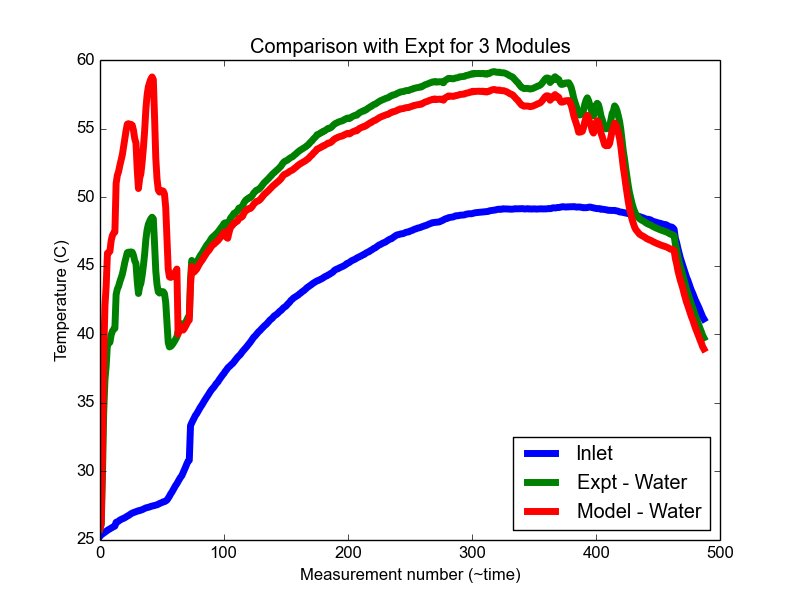
\includegraphics[width=0.6\textwidth]{nov25.png}
\caption{Comparison between experiment and model for 3 modules, water temperature in last module compared.}
\end{figure}
\begin{figure}[!ht]
\centering
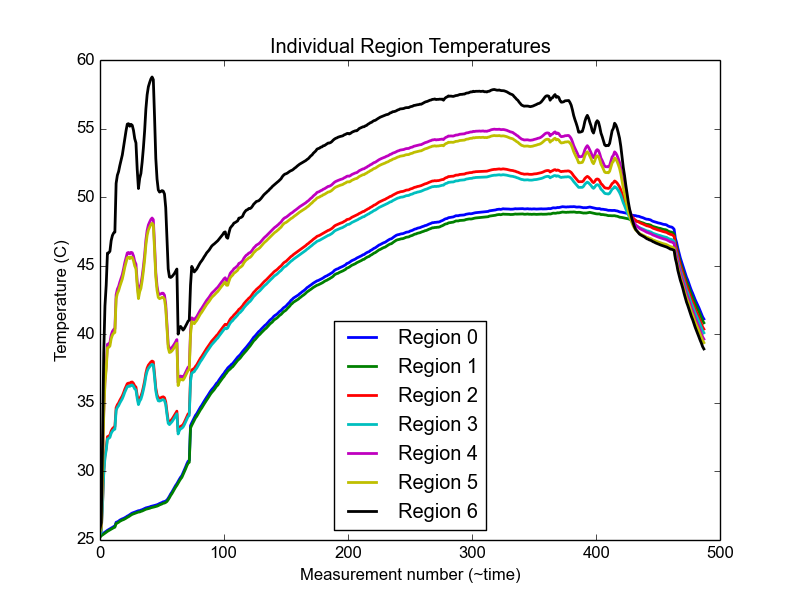
\includegraphics[width=0.6\textwidth]{nov25modules.png}
\caption{Model results for 3 module case, using experimental inputs. Regions 2,4,6 correspond to modules.}
\end{figure}
\subsection{Feb 11 data}
\begin{figure}[!ht]
\centering
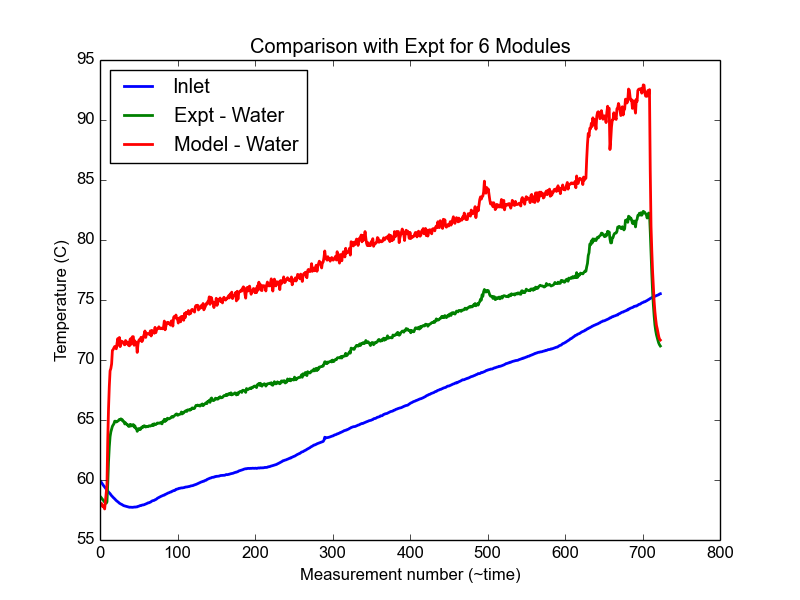
\includegraphics[width=0.6\textwidth]{feb11.png}
\caption{Comparison between experiment and model for 6 modules, water temperature in last module compared for Feb 11th data. Each module has its own $Q_w$ from the data.}
\end{figure}

\begin{figure}[!ht]
\centering
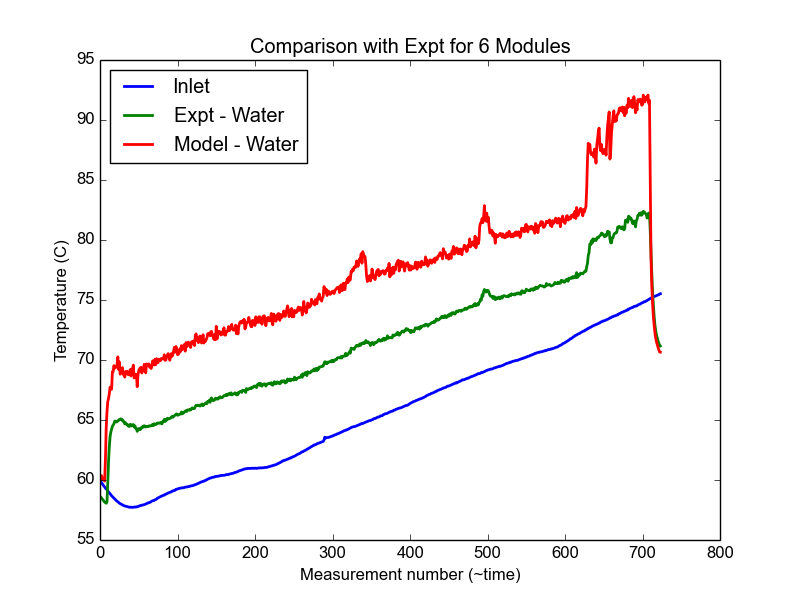
\includegraphics[width=0.6\textwidth]{feb11_oneblock.png}
\caption{Same Comparison, in this case, regions 1-2, 3-4, etc are merged into one, as if the module is part of the general volume.}
\end{figure}
\begin{figure}[!ht]
\centering
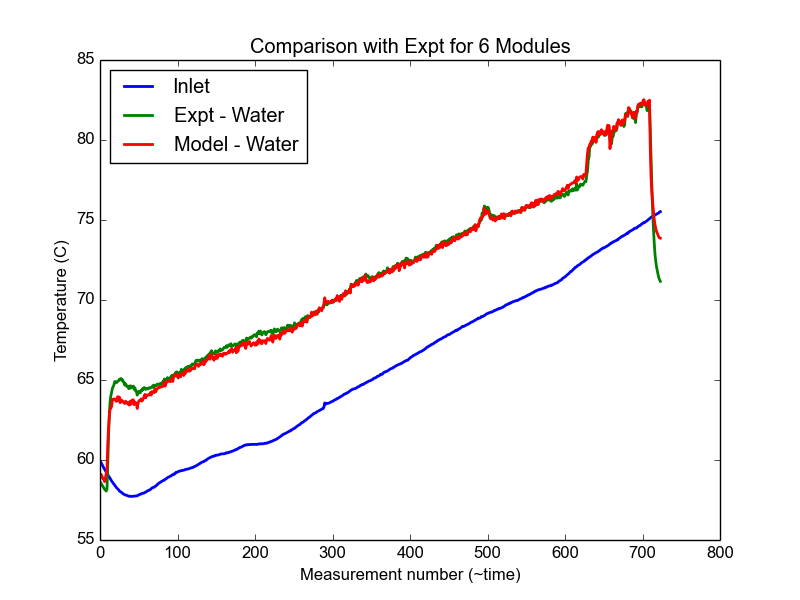
\includegraphics[width=0.6\textwidth]{feb11_2_4water.png}
\caption{Same Comparison. In the model, the water flow rate is 2.4 times the number initially used. This gets closer to the experimental data.}
\end{figure}
\begin{figure}[!ht]
\centering
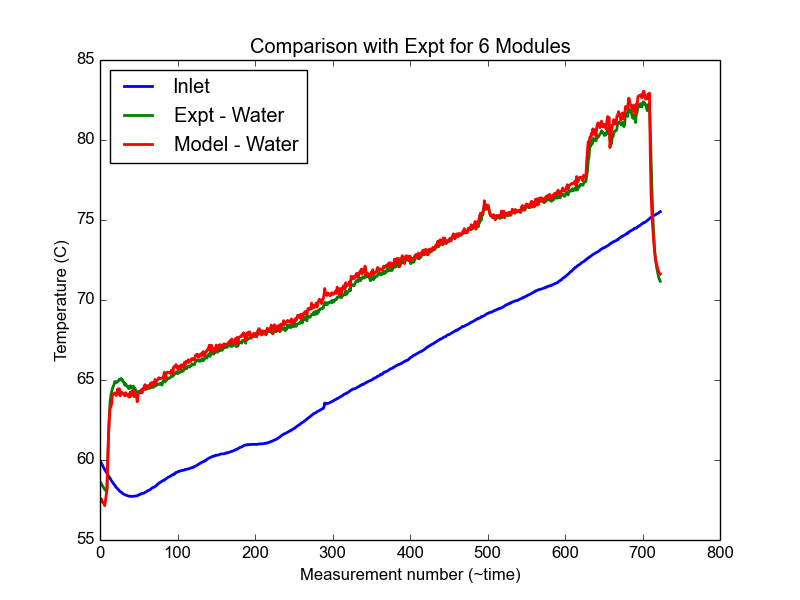
\includegraphics[width=0.6\textwidth]{feb11_55.png}
\caption{Same Comparison. In the model, the heat generated, $Q_w$ in each module is 55\% of the experimental number, suggesting better agreement if there is a loss of energy.}
\end{figure}
\clearpage
\newpage 
\section{Unsteady Model}
Consider the steady model in \ref{eq:steady} and introduce the time derivative, $mC_{p}\frac{\partial T}{\partial t}$ and rearrange to get 
\begin{eqnarray} 
W_1: & & m_{w,1}C_{p,w}\frac{\partial T}{\partial t} + \dot{m}_wC_{p,w}(T_{w,1}-T_{w,0}) - h_{wa}(T_{a,1}-T_{w,1}) = 0 \\
W_2: & & m_{w,2}C_{p,w}\frac{\partial T}{\partial t} + \dot{m}_wC_{p,w}(T_{w,2}-T_{w,1}) - Q_w(t) = 0\\
A_1: & & m_{a,1}C_{p,a}\frac{\partial T}{\partial t} + \dot{m}_aC_{p,a}(T_{a,1}-T_{a,0}) - h_{wa}(T_{w,1}-T_{a,1}) - h_{e}(T_e-T_{a,1}) - h_{i}(T_i-T_{a,1})= 0 \\
A_2: & & m_{a,2}C_{p,a}\frac{\partial T}{\partial t} +\dot{m}_aC_{p,a}(T_{a,2}-T_{a,1}) - Q_a = 0 
\end{eqnarray}
To handle the mass term, we need the volume. We have a length of the first tube as $L_1 = 0.15m$ and $L_{3,5,\ldots} = 0.3m$. The cross sectional area of the tube is based on inner diameter, $d = 0.003m$ and outer diameter of $d = 0.0142m$. The volume of the surrounding air we are interested in has a cross section of $0.4m \times 0.4m$. Using the density and the specific heat, we get that $m_a = 0.0576 kg$, $m_w = 2.12\times 10^{-3} kg$.

For regions with modules, we can create a small volume, $m_{a,2,4,6,\ldots} \approx Cm_a$ and $m_{w,2,4,6,\ldots} Cm_w$. In these results, $C = 1/6$.

\subsection{Feb 11 data}
Using the Feb 11 data, given discrete data, we can determine $Q_w(t)$ for all times by quadratic interpolation. For the initial solution, we can set every 

\begin{figure}[!ht]
\centering
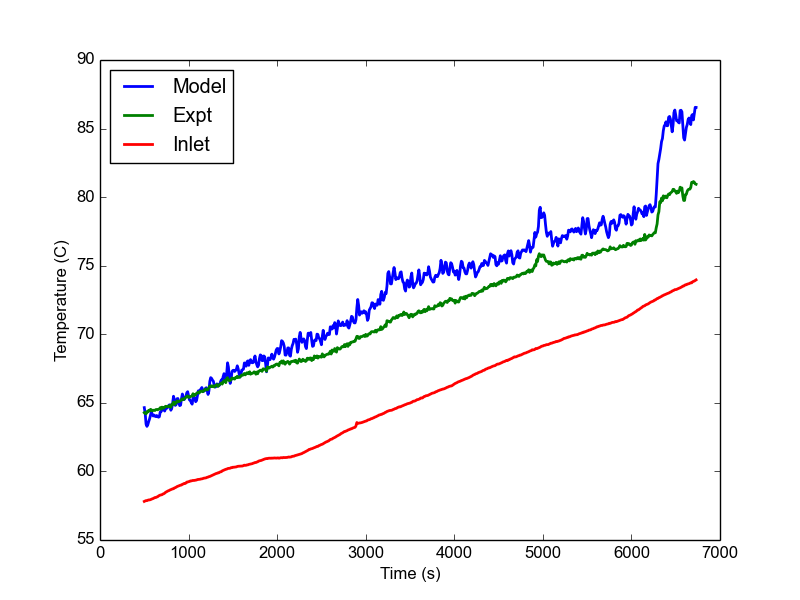
\includegraphics[width=0.6\textwidth]{Feb11_unst_10.png}
\caption{Same Comparison. In the model, the heat generated, $Q_w$ in each module is 65\% of the experimental number. Initially they start out in agreement, and then diverge as time goes on. Quadratic interpolation of the data (inlet temp, heat generated).}
\end{figure}
\end{document}

